\documentclass[11pt,a4paper]{article}
\usepackage[utf8]{inputenc}\usepackage[T1]{fontenc}
\usepackage[margin=1in]{geometry}
\usepackage{amsmath,amssymb,booktabs,graphicx,enumitem,xcolor,parskip,titlesec}
\usepackage[hidelinks]{hyperref}
\graphicspath{{figures/}}
\definecolor{qnavy}{RGB}{20,40,75}\definecolor{qgrey}{RGB}{90,90,90}\definecolor{qred}{RGB}{150,30,30}
\titleformat{\section}{\large\bfseries\color{qnavy}}{\thesection}{0.6em}{}
\begin{document}\thispagestyle{empty}
\noindent
{\large\bfseries\color{qnavy} Report R05 --- Imaging versus Molecular Markers, Head to Head}\\[2pt]
{\color{qgrey}Same patients, same folds. Partly walks back R02.}\\[6pt]
{\color{qgrey}\rule{\textwidth}{0.4pt}}

\medskip
\noindent 7 August 2026 \quad\textbullet\quad Quantara

\section*{Summary}

R02 measured imaging on UPENN-GBM and R04 measured molecular markers on TCGA and MSK, so the
two were matched on disease but not on population. This report removes that gap by running
both on the \textbf{same 247 UPENN patients} who have radiomic features, survival, and
definite IDH1 and MGMT calls.

\textbf{Imaging does not add established prognostic value beyond MGMT in this subset.}
Across eight cross-validation seeds the likelihood-ratio test for adding the radiomic score
to a molecular model gives a median $p = 0.089$, clearing 0.05 in only \textbf{2 of 8}
seeds. Imaging alone reaches C-index 0.512--0.549 here, against 0.573 for the molecular
model. Conversely, molecular markers add to imaging decisively
($\chi^2_2 = 33.7$, $p = 4.8\times10^{-8}$).

Two honest qualifications follow, and both are consequences of the audit rather than the run.

\section{Results}

\begin{center}
\begin{tabular}{@{}lc@{}}
\toprule
\textbf{Predictor (same 247 patients, same folds)} & \textbf{Cross-validated C-index} \\
\midrule
Molecular (IDH1 $+$ MGMT) & 0.573 \\
Imaging alone & 0.524 \quad{\footnotesize(0.512--0.549 across seeds)} \\
Combined & 0.591 \\
Combined $+$ age & \textbf{0.642} \\
\bottomrule
\end{tabular}
\end{center}

\begin{center}
\begin{tabular}{@{}lccl@{}}
\toprule
\textbf{Incremental value} & \textbf{$\chi^2$} & \textbf{$p$} & \textbf{Verdict} \\
\midrule
Imaging beyond molecular & 3.71 (df 1) & 0.054 single seed; \textbf{median 0.089} & not established \\
Molecular beyond imaging & 33.69 (df 2) & $4.8\times10^{-8}$ & decisive \\
\bottomrule
\end{tabular}
\end{center}

\noindent Cox terms in the combined model: MGMT HR 0.473 ($p=1.2\times10^{-7}$),
radiomic score HR 0.881 ($p=0.055$), IDH1 HR 0.591 ($p=0.254$).

\begin{center}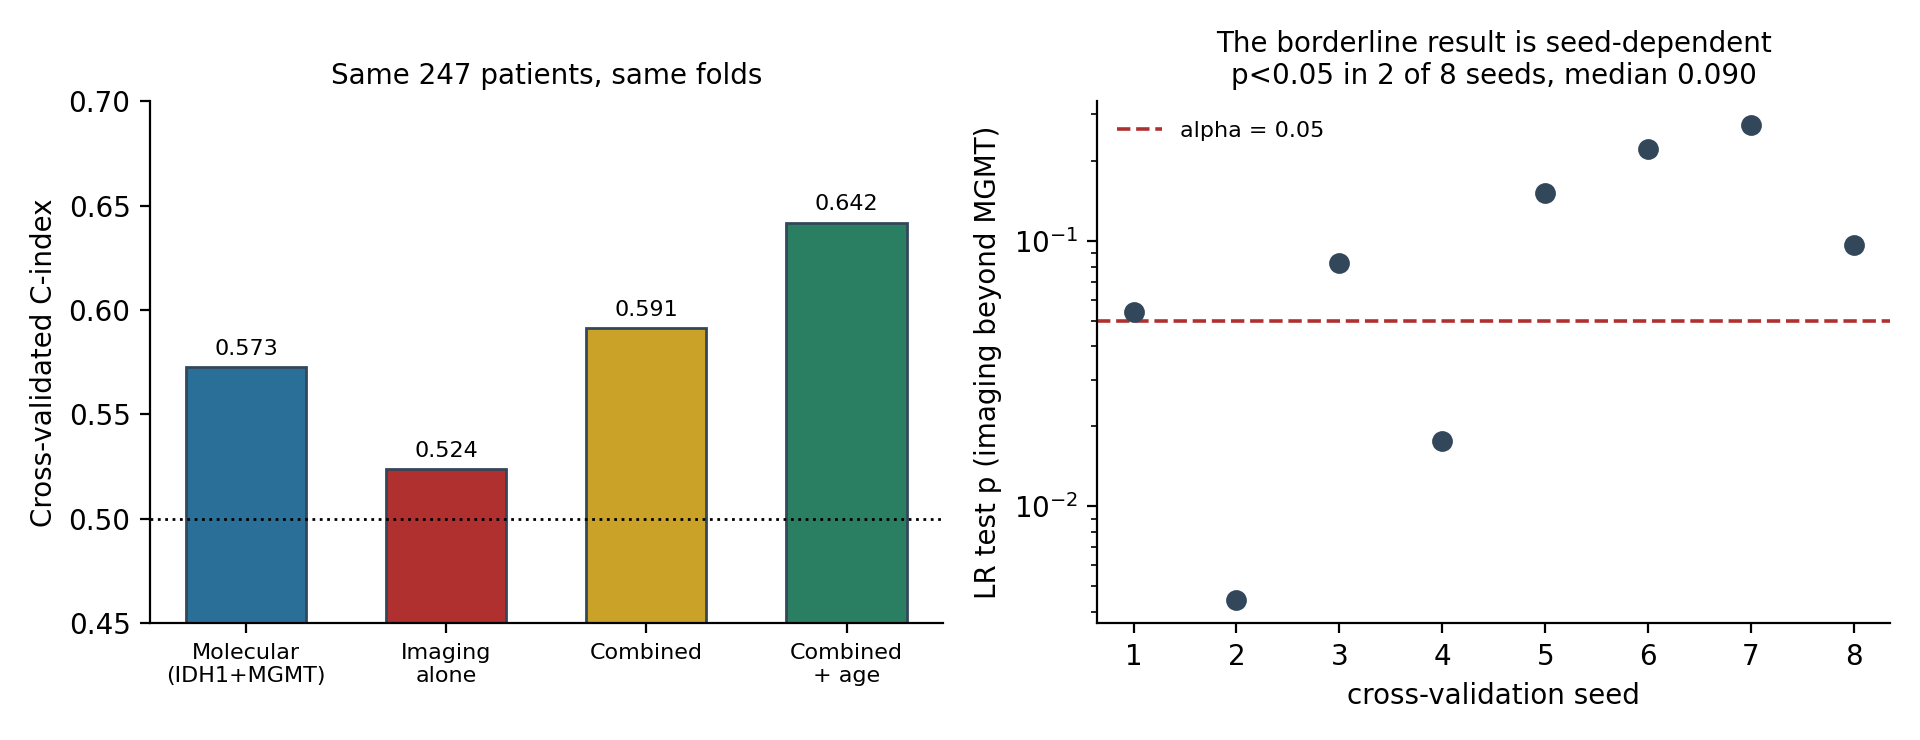
\includegraphics[width=\textwidth]{fig1_head2head.png}\end{center}

\section{\textcolor{qred}{Two qualifications the audit forced}}

\textbf{1. The ``molecular panel'' is MGMT alone.} Only \textbf{5 of 247} patients are
IDH1-mutant --- expected, since UPENN is a glioblastoma cohort. Adding IDH to MGMT changes
nothing ($\chi^2=1.45$, $p=0.228$). Every statement above about ``molecular markers'' should
be read as ``MGMT''.

\textbf{2. The single $p=0.054$ was coincidental, and we should not have relied on it.} The
audit re-derived the radiomic score under eight cross-validation seeds; the LR $p$ ranged
from 0.0045 to 0.274. Reporting one draw near the threshold would have been misleading in
either direction. The seed distribution is the result.

The underlying cause is an inconsistency of ours: R02 used $10\times$ repeated 5-fold with
averaged predictions, while R05 used a single 5-fold. R02's protocol was the more robust
one. A repeated-CV rerun is the clean fix and is recommended before this analysis appears in
any manuscript.

\section{Reconciling with R02}

R02 reported imaging C-index 0.602 on 574 patients; here it is $\approx$0.535 on 247. The
subset requires a definite MGMT call and is 43\% of the size. R02's estimate remains the
better one \emph{for its cohort}; R05's is the better one \emph{for the head-to-head
question}. Neither supersedes the other and the discrepancy is stated rather than smoothed
over.

\section{What this means for the glioma arm}

Taken with R04, the position is now specific and defensible, and less optimistic than R02
alone suggested:

\begin{itemize}[leftmargin=1.4em,nosep]
\item Within glioblastoma, \textbf{MGMT is the strongest single prognostic variable we hold},
and age adds substantially on top (0.591 $\to$ 0.642).
\item Imaging carries \emph{some} prognostic signal (R02, $p=0.005$ against a correctly
centred null, independent of age) but \textbf{its incremental value over MGMT is not
established} at this sample size.
\item The claim worth making is therefore modest: radiomics is prognostically informative in
glioblastoma, not that it improves on standard molecular assessment.
\end{itemize}

\section{Audit}

\begin{center}
\begin{tabular}{@{}llp{7.0cm}@{}}
\toprule
\textbf{Check} & \textbf{Verdict} & \textbf{Finding} \\
\midrule
Positive control (MGMT) & \textbf{Recovered} & median 595 vs 371 days, $p=5.8\times10^{-8}$ \\
Is the panel two markers? & \textbf{No} & IDH mutant $n=5$; adding IDH $p=0.228$ \\
Is $p=0.054$ stable? & \textbf{No} & 8 seeds: 0.0045--0.274, median 0.089, 2/8 below 0.05 \\
Method consistency & \textbf{Our inconsistency} & R02 used repeated CV; R05 a single split \\
Gates & \textbf{4 / 4 PASS} & Integrity, cohort size, uncensored, positive control \\
\bottomrule
\end{tabular}
\end{center}

\section{How to verify}

\texttt{evidence/head2head.csv} carries survival days, IDH1, MGMT, the radiomic score and age
for all 247 patients --- every C-index and Cox model above is recomputable from it.
\texttt{audit\_seed\_stability.json} holds all eight seed results.
\texttt{config.yaml} (hash \texttt{70713fdd\ldots}) was written before any outcome was read.

\vfill
\noindent{\color{qgrey}\rule{\textwidth}{0.4pt}}\\
{\footnotesize\color{qgrey}Run \texttt{runs/20260806T235753Z-R05head2head-3f8bece}. Data:
UPENN-GBM, TCIA, CC BY 4.0. No patient-level identifiers reproduced.}
\end{document}
